\documentclass[30pt,twocolumn,letterpaper]{article}
\usepackage{cvpr}
\usepackage{times}
\usepackage{booktabs}
\usepackage{epsfig}
\usepackage{graphicx}
\usepackage{amsmath}
\usepackage{amssymb}
\cvprfinalcopy
\def\cvprPaperID{****}
\def\httilde{\mbox{\tt\raisebox{-.5ex}{\symbol{126}}}}
\usepackage{graphicx}
\usepackage{indentfirst}
\setlength{\parindent}{2em}
\usepackage{cite}
\usepackage[colorlinks,linkcolor=red,anchorcolor=blue,citecolor=green,backref=page]{hyperref}
\author{Qilei Zhang\\\\
Jul 16 2018}
\title{Landmarks-based Kernelized Subspace Alignment for Unsupervised Domain Adaptation}
\begin{document}
\maketitle
\begin{abstract}
  Domain adaptation has achieved great success in computer vision in recent years, in order to process the learning process to transfer knowledge from the source to the target domain. In this article, we introduce a new unsupervised DA method based on subspace alignment and selection of landmarks, which are also distributed between two domains. These landmarks are selected to reduce the differences between domains, and then used to projecting data in the same space, in which the effective subspace alignment is performed in a closed form.
\end{abstract}
\section{Introduction}
While the standard machine learning setting assumes that training and test data come from the same statistical distribution, it turns out that many real world applications, in Computer Vision or in Natural Language Processing, challenge this assumption\cite{Wu2014Learning}. Indeed, the data from which the classifier is supposed to be learned often differ from the target data the classifier will be deployed on Figure 1. To deal with such situations, the learning system has to take into account the distribution shift between the two domains in order to adapt well from the source to the target. In this framework, two main categories of domain adaptation methods are available\cite{Sun2016Discriminative}. \\
\begin{figure}[htbp]
\small
\centering
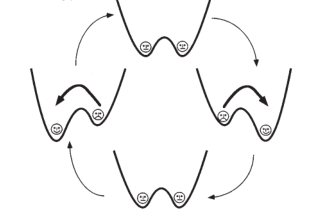
\includegraphics[width=20em]{000.png}
\caption{Example of distribution shift between images from two
datasets. First row, some bike helmets from the Amazon subset
and second row, bike helmets from the webcam subset. These 2
subsets are from the Office dataset.
}
\label{fig:lable}
\end{figure}\\
\section{Related Work}
Domain adaptation is one of the possible settings for transfer learning. In the article, we focus on the most complex case, called unsupervised DA, where the label data can only be from the source domain. In this case, in order to reduce the offset between the source and the target distribution, a strategy includes weighting each source data based on the similarity between the source data and the target domain\cite{Khuller1996Landmarks}.
\begin{figure}[htbp]
\small
\centering
\includegraphics[width=20em]{001.png}
\caption{(Best shown in color) Domain adaptation problem that
needs to adapt a source (S) domain to a target (T) domain w.r.t.
four classes of examples (green, orange, blue and red). We can
see that no linear transformation will be able to entirely bridge
the source to the target. On the other hand, we can note that, for
each class, some subsets of source and target examples seem to be
similarly distributed (in black). The objective is to automatically
discover those so-called landmarks that will be used to map both
source and target data onto a common space using a kernel.
}
\label{fig:lable}
\end{figure}\\
\section{Conclusion}
The DA method based on subspace alignment has attracted much interest recently. In this framework, the most accurate method assumes that the offset between source and target distributions can be corrected by linear functions\cite{Yu2012Image}. However, experiments show that this assumption is challenged in most real-world applications. Therefore, nonlinear mapping functions should be optimized for homogeneous sources and target subspaces. Moreover, there is no reason to prove that the constrained DA algorithm adapts all training source data to the target domain\cite{Fabbri2016Multiview}.\\
{\small
\bibliographystyle{ieee}
\bibliography{1}
}
\end{document}
